\documentclass[a4paper,12pt]{article}
\usepackage[polish]{babel}
\usepackage[utf8]{inputenc}
\usepackage{amsfonts}
\usepackage{indentfirst}
\usepackage[T1]{fontenc}
\usepackage{amsmath}
\usepackage{hyperref}
\usepackage{graphicx}
\usepackage{subcaption}
\usepackage{fancyvrb}
\usepackage{wrapfig}
\usepackage[toc,page]{appendix} % for appendix

\textwidth\paperwidth
\advance\textwidth -45mm
\oddsidemargin 18mm
\advance\oddsidemargin -18mm
\evensidemargin 18mm
\advance\evensidemargin -18mm
\topmargin -30mm
\advance\topmargin 17mm
\setlength\textheight{45\baselineskip}
\addtolength\textheight{\topskip}
\marginparwidth 15mm

\addto\captionspolish{ % rename Appendices title to Dodatki
\renewcommand\appendixname{Dodatek}
\renewcommand\appendixpagename{Dodatki}
}


\title{
Zaawansowane metody uczenia maszynowego \\
Projekt 2
}
\author{
Mikołaj Małkiński \\
\texttt{malkinskim@student.mini.pw.edu.pl}
}
\date{\today}

\begin{document}
    \maketitle

    \section{Wstępna analiza danych}

    \begin{wrapfigure}{r}{0.5\linewidth}
        \centering
        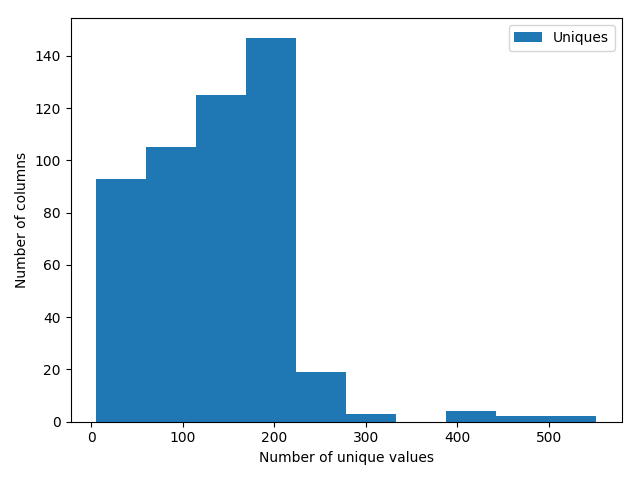
\includegraphics[width=\linewidth]{../images/uniqueness-train.png}
        \caption{Unikalne wartości}
        \label{fig:uniqueness-train}
    \end{wrapfigure}

    Oryginalny zbiór danych został podzielony na treningowy (2000 obserwacji) oraz testowy (600 obserwacji).
    Oba zbiory zawierają 500 kolumn numerycznych.
    Zbiory nie posiadają żadnych brakujących wartości.
    Rysunek~\ref{fig:uniqueness-train} przedstawia stosunek liczby unikalnych wartości w kolumnie, dla liczby kolumn.

    Na początku, porównano rozkłady zmiennych ze względu na zbiór danych (Dodatek~\ref{appendix:rozklad-cech-numerycznych-zbiory}) oraz klasę (Dodatek~\ref{appendix:rozklad-cech-numerycznych-klasy}).
    Wyraźnie można zauważyć że zmienne zostały wygenerowane z rozkładów normalnych z różną średnią i odchyleniem standardowym.
    Podział ze względu na zbiór dla niektórych zmiennych pokazuje delikatne różnice, jednak wynika to prawdopodobnie z małych rozmiarów zbiorów.
    Natomiast, podział ze względu na klasę nie ujawnił żadnych widocznych różnic.

    \begin{table}
        \hspace*{-1cm}
        \begin{tabular}{l|*{6}{c}}
            & AUC & Dokładność & Zbalansowana dok. & F1 & Precyzja & Czułość \\
            \hline
            XGBoost & 0.8309 & 0.7400 & 0.7390 & 0.7249 & 0.7366 & 0.7135 \\
            LightGBM & \textbf{0.8791} & \textbf{0.8025} & \textbf{0.8023} & \textbf{0.7948} & \textbf{0.7927} & \textbf{0.7969} \\
            AdaBoost & 0.6227 & 0.6125 & 0.6138 & 0.6154 & 0.5877 & 0.6458 \\
            GradientBoosting & 0.8159 & 0.7275 & 0.7272 & 0.7169 & 0.7150 & 0.7188 \\
            RandomForest & 0.6781 & 0.6475 & 0.6446 & 0.6094 & 0.6509 & 0.5729 \\
            ExtraTrees & 0.5691 & 0.5575 & 0.5549 & 0.5151 & 0.5434 & 0.4896 \\
        \end{tabular}
        \hspace*{1cm}
        \caption{Metryki podstawowych modeli klasyfikacyjnych}
        \label{tab:score-comparison}
    \end{table}

    \section{Podstawowe modele w domyślnych konfiguracjach}

    \begin{wrapfigure}{l}{0.5\linewidth}
        \centering
        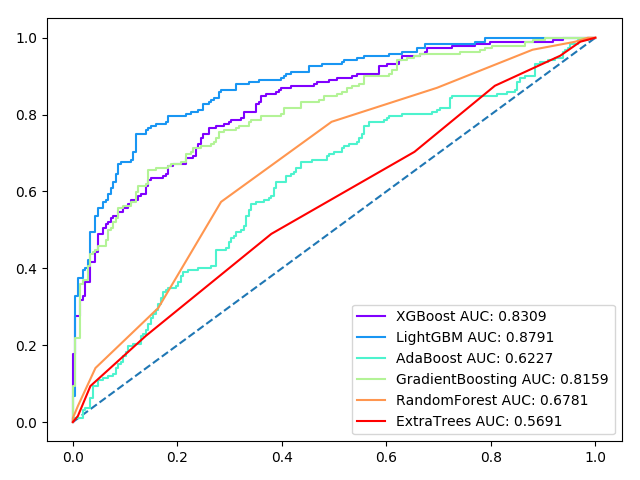
\includegraphics[width=\linewidth]{../images/roc-comparison.png}
        \caption{Porównanie krzywych ROC podstawowych modeli klasyfikacyjnych}
        \label{fig:roc-comparison}
    \end{wrapfigure}

    Po odpowiednim przygotowaniu danych, w prosty sposób można sprawdzić jakość różnych modeli z domyślnymi parametrami.
    Zbiór danych został podzielony na treningowy i walidacyjny w stosunku 4:1.
    Zbadano jakość następujących klasyfikatorów: \textit{XGBoost}~\cite{xgboost}, \textit{LightGBM}~\cite{lightgbm}, \textit{AdaBoost}~\cite{adaboost}, \textit{GradientBoosting}~\cite{gradient-boosting}, \textit{RandomForest}~\cite{random-forest}, \textit{ExtraTrees}~\cite{extra-trees}.

    Krzywe ROC tych modeli zaprezentowane są na Rysunku~\ref{fig:roc-comparison}.
    Łatwo zauważyć rozbieżność w otrzymanych krzywych ROC\@.
    Przypuszcza się, że jest to spowodowane dużą liczbą nieistotnych kolumn w zbiorze danych - niektóre z użytych modeli nie są w stanie dobrze wybrać wartościowe kolumny.
    Najlepsze wyniki osiągnęły modele LightGBM oraz XGBoost, więc to one zostaną użyte do przeprowadzenia kolejnych eksperymentów.
    Dokładniejsze statystki przedstawione są w Tablicy~\ref{tab:score-comparison}.
    Porównano w niej takie metryki jak: AUC, dokładność, zbalansowaną dokładność, F1, precyzję oraz czułość.

    \section{Wybór cech}

    Oryginalny zbiór danych posiadał 500 kolumn numerycznych.
    Aby ograniczyć ich liczbę, wybrano te, które są najważniejsze do dokonania poprawnej klasyfikacji.
    Zmniejszenie liczby zmiennych przede wszystkim pomaga zmniejszeniu zjawiska przetrenowania, co pozytywnie wpływa na dokładność klasyfikacji, oraz znacząco redukuje czas trenowania.
    W tej sekcji zostały opisane metody które zostały wykorzystane do ostatecznego wyboru zmiennych.

    \begin{wrapfigure}{r}{0.4\linewidth}
        \vspace{-40pt}
        \centering
        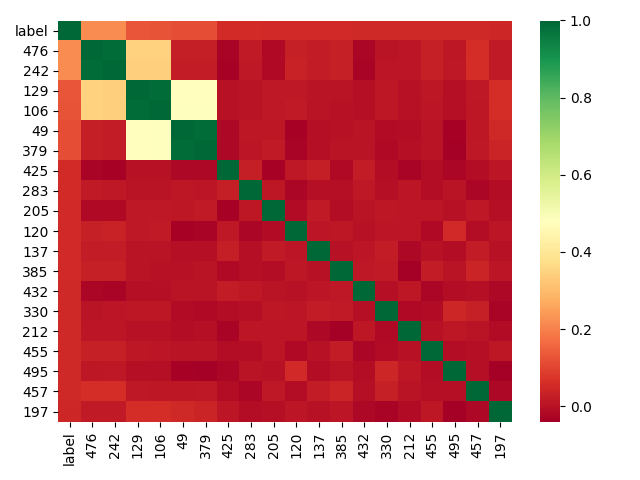
\includegraphics[width=\linewidth]{../images/correlation-matrix.png}
        \caption{Macierz korelacji ograniczona do 20 największych wartości}
        \label{fig:correlation-matrix}
    \end{wrapfigure}

    \subsection{Macierz korelacji}\label{subsec:macierz-korelacji}

    Pierwszym sposobem było zbadanie korelacji między zmiennymi.
    Wynik dla 20 zmiennych zawierających najwyższe wartości zaprezentowany jest na Rysunku~\ref{fig:correlation-matrix}.
    Wizualizacja pokazuje że korelacja jest mała, jednak warto zwrócić uwagę na zmienne: 476, 242, 129, 106, 49 oraz 379.
    Pomimo tego że wybrane pary są ze sobą wyraźnie bardziej skorelowane niż inne, to są one także zależne od zmiennej \textit{label}, która określa klasę do której przynależy dana obserwacja.
    Eksperymenty omówione w Sekcji~\ref{subsec:rekurencyjna-eliminacja-cech} wykazały że zmienne z wyjątkiem 129 zostały wybrane w jednym bądź obu przypadkach.

    \begin{wrapfigure}{r}{0.5\linewidth}
        \vspace{-40pt}
        \centering
        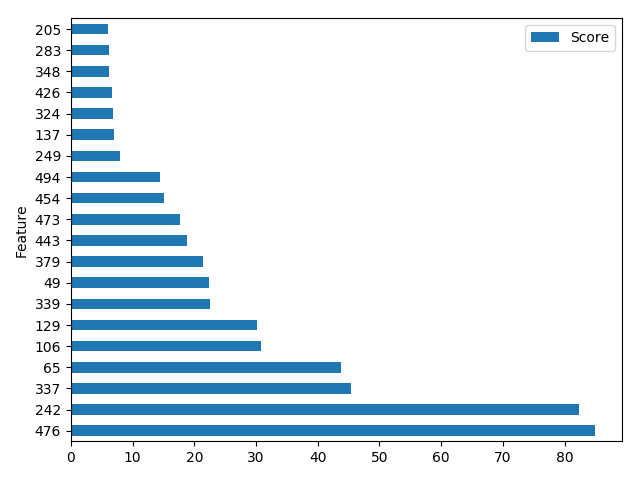
\includegraphics[width=\linewidth]{../images/univariate-selection.png}
        \caption{20 największych wartości otrzymanych za pomocą testu ANOVA}
        \label{fig:univariate-selection}
    \end{wrapfigure}

    \subsection{Analiza jednowymiarowa}\label{subsec:wybor-jednowymiarowy}

    Kolejną metodą było przeprowadzonenie testu statystycznego, który osobno sprawdzał zależność między każdą zmienną a zmienną określającą przynależność do danej klasy.
    Zmienne zostały wybrane na podstawie F-wartości osiągniętej z testu ANOVA (analiza wariancji).
    Rysunek~\ref{fig:univariate-selection} przedstawia otrzymane wyniki.
    Warto zwrócić uwagę, że ponownie wyróżniły się zmienne 476, 242, 106, 129, 49 oraz 379, które zostały wyszczególnione w Sekcji~\ref{subsec:macierz-korelacji}.
    Dodatkowo, dobre wyniki osiągnęły zmienne 337, 339, 443, 473 oraz 454, które także pojawią się w Sekcji~\ref{subsec:rekurencyjna-eliminacja-cech}.

    \subsection{Rekurencyjna eliminacja cech}\label{subsec:rekurencyjna-eliminacja-cech}

    Oba modele, LightGBM oraz XGBoost, po zakończonym treningu są w stanie określić które cechy są najbardziej istotne dla wytrenowanego modelu.
    Wykresy pokazujące przykładowy ranking przedstawione są w Dodatkach~\ref{appendix:feature-importance-lightgbm} oraz~\ref{appendix:feature-importance-xgboost}.
    Na podstawie takich metryk, przeprowadzona została eliminacja cech, używając 5-krotnej kroswalidacji.
    Polega ona na wielokrotnym trenowaniu modelu, usuwając najmniej istotne cechy po każdej iteracji.
    Rysunek~\ref{fig:rfe-cv-comparison} przedstawia zbalansowaną dokładność modeli LightGBM oraz XGBoost w zależności od ilości wykorzystanych cech.
    W pierwszym przypadku, najlepszy wynik został osiągnięty korzystając z 7 cech (106, 154, 319, 337, 379, 443, 454), a w drugim korzystając z 13 cech (29, 49, 106, 154, 242, 282, 319, 339, 379, 443, 452, 473, 476).
    Wyraźnie widać że wykorzystane cechy zostały już zauważone w Sekcjach~\ref{subsec:macierz-korelacji} oraz~\ref{subsec:wybor-jednowymiarowy}.

    \begin{figure}[h!]
        \centering
        \begin{subfigure}{0.5\linewidth}
            \centering
            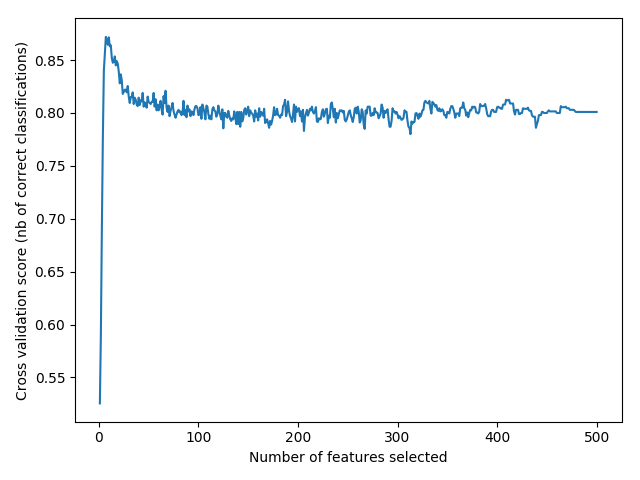
\includegraphics[width=0.9\linewidth]{../images/lightgbm-rfe-cv.png}
            \caption{LightGBM}
        \end{subfigure}%
        ~
        \begin{subfigure}{0.5\linewidth}
            \centering
            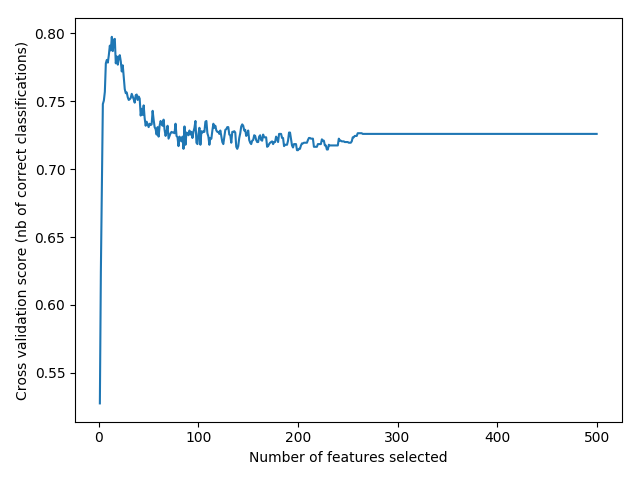
\includegraphics[width=0.9\linewidth]{../images/xgboost-rfe-cv.png}
            \caption{XGBoost}
        \end{subfigure}
        \caption{Zbalansowana dokładność w zależności od liczby zmiennych}
        \label{fig:rfe-cv-comparison}
    \end{figure}

    \section{Dobór hiperparametrów}

    Następnie, dla obu modeli LightGBM oraz XGBoost dokonano doboru hiperparametrów korzystając z 5-krotnej kroswalidacji, tak aby osiągnąć jak najwyższą zbalansowaną dokładność.
    Dla każdego z modeli użyto innego zbioru danych, złożonego tylko z cech które zostały wybrane dla danego modelu w Sekcji~\ref{subsec:rekurencyjna-eliminacja-cech}.
    LightGBM, korzystając z 7 cech, osiągnął średnią zbalansowaną dokładność równą 87.2\%, a XGBoost, korzystając z 13, równą 85.9\%.
    Na tej podstawie, do ostatecznej predykcji klas dla zbioru testowego użyto modelu LightGBM\@.

    \bibliographystyle{plain}
    \bibliography{report}

    \newpage
    \begin{appendices}

        \section{Rozkład cech z podziałem na zbiór}\label{appendix:rozklad-cech-numerycznych-zbiory}

        \begin{figure}[!h]
            \centering
            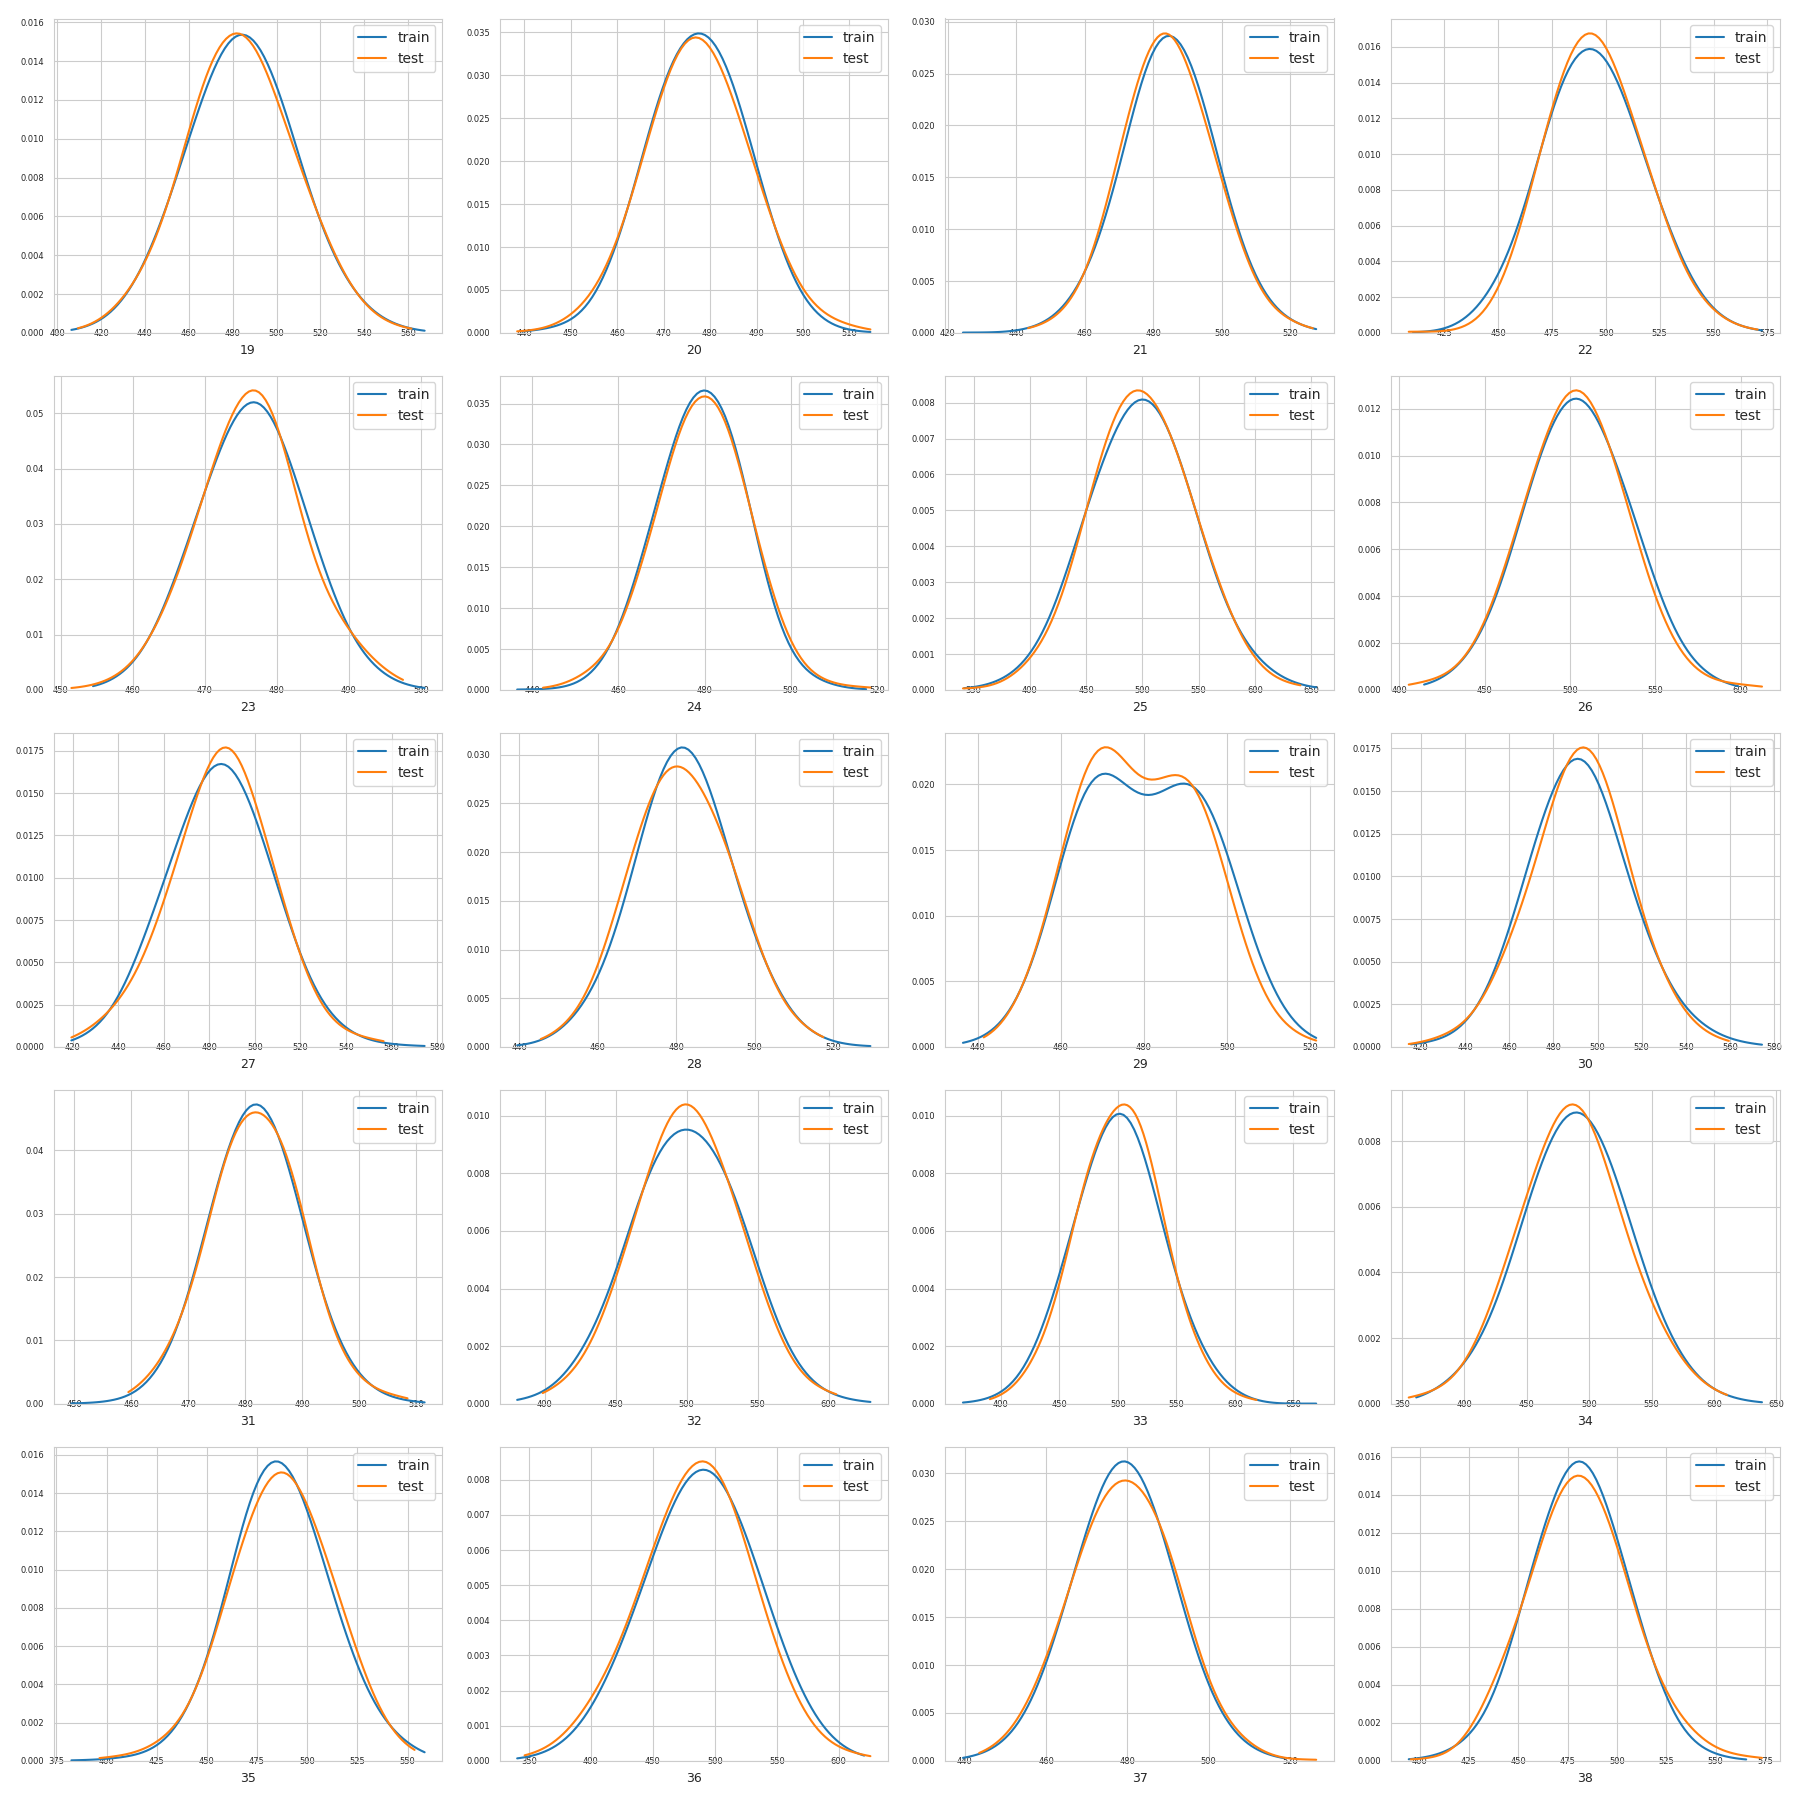
\includegraphics[width=0.9\textwidth]{../images/feature-distribution-dataset.png}
            \caption{Rozkład cech z podziałem na zbiór}
        \end{figure}

        \newpage

        \section{Rozkład cech z podziałem na klasę}\label{appendix:rozklad-cech-numerycznych-klasy}

        \begin{figure}[!h]
            \centering
            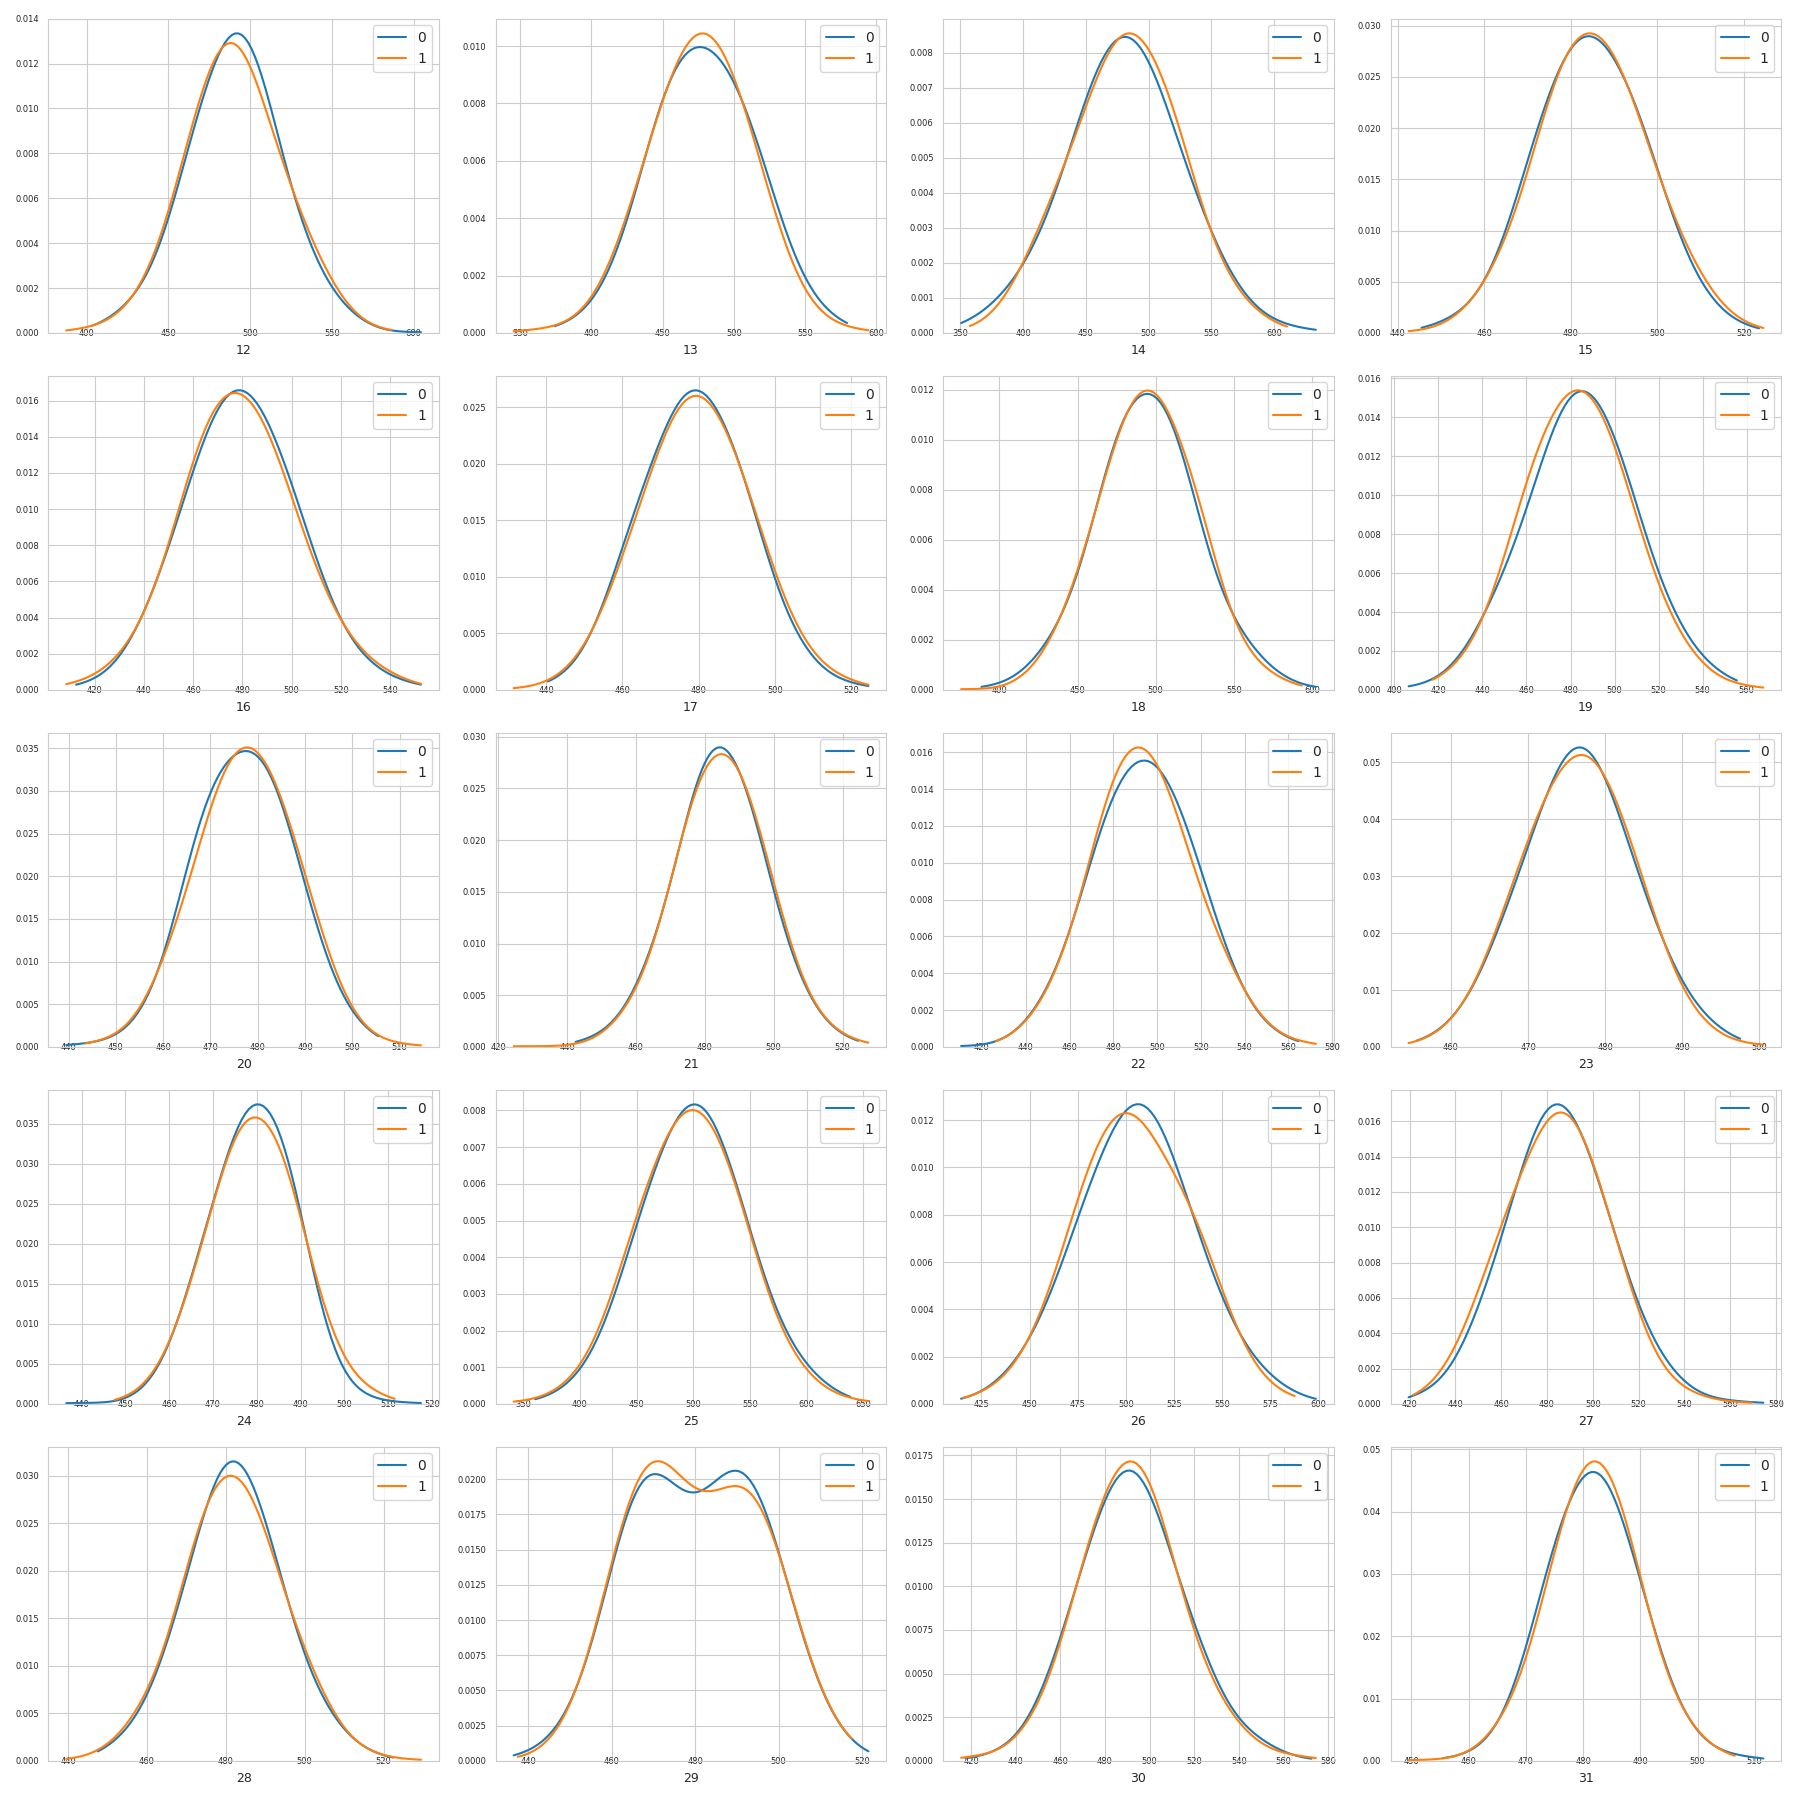
\includegraphics[width=0.9\textwidth]{../images/feature-distribution-label.png}
            \caption{Rozkład cech z podziałem na klasę}
        \end{figure}

        \newpage

        \section{Istotność cech dla modelu LightGBM}\label{appendix:feature-importance-lightgbm}

        \begin{figure}[!h]
            \centering
            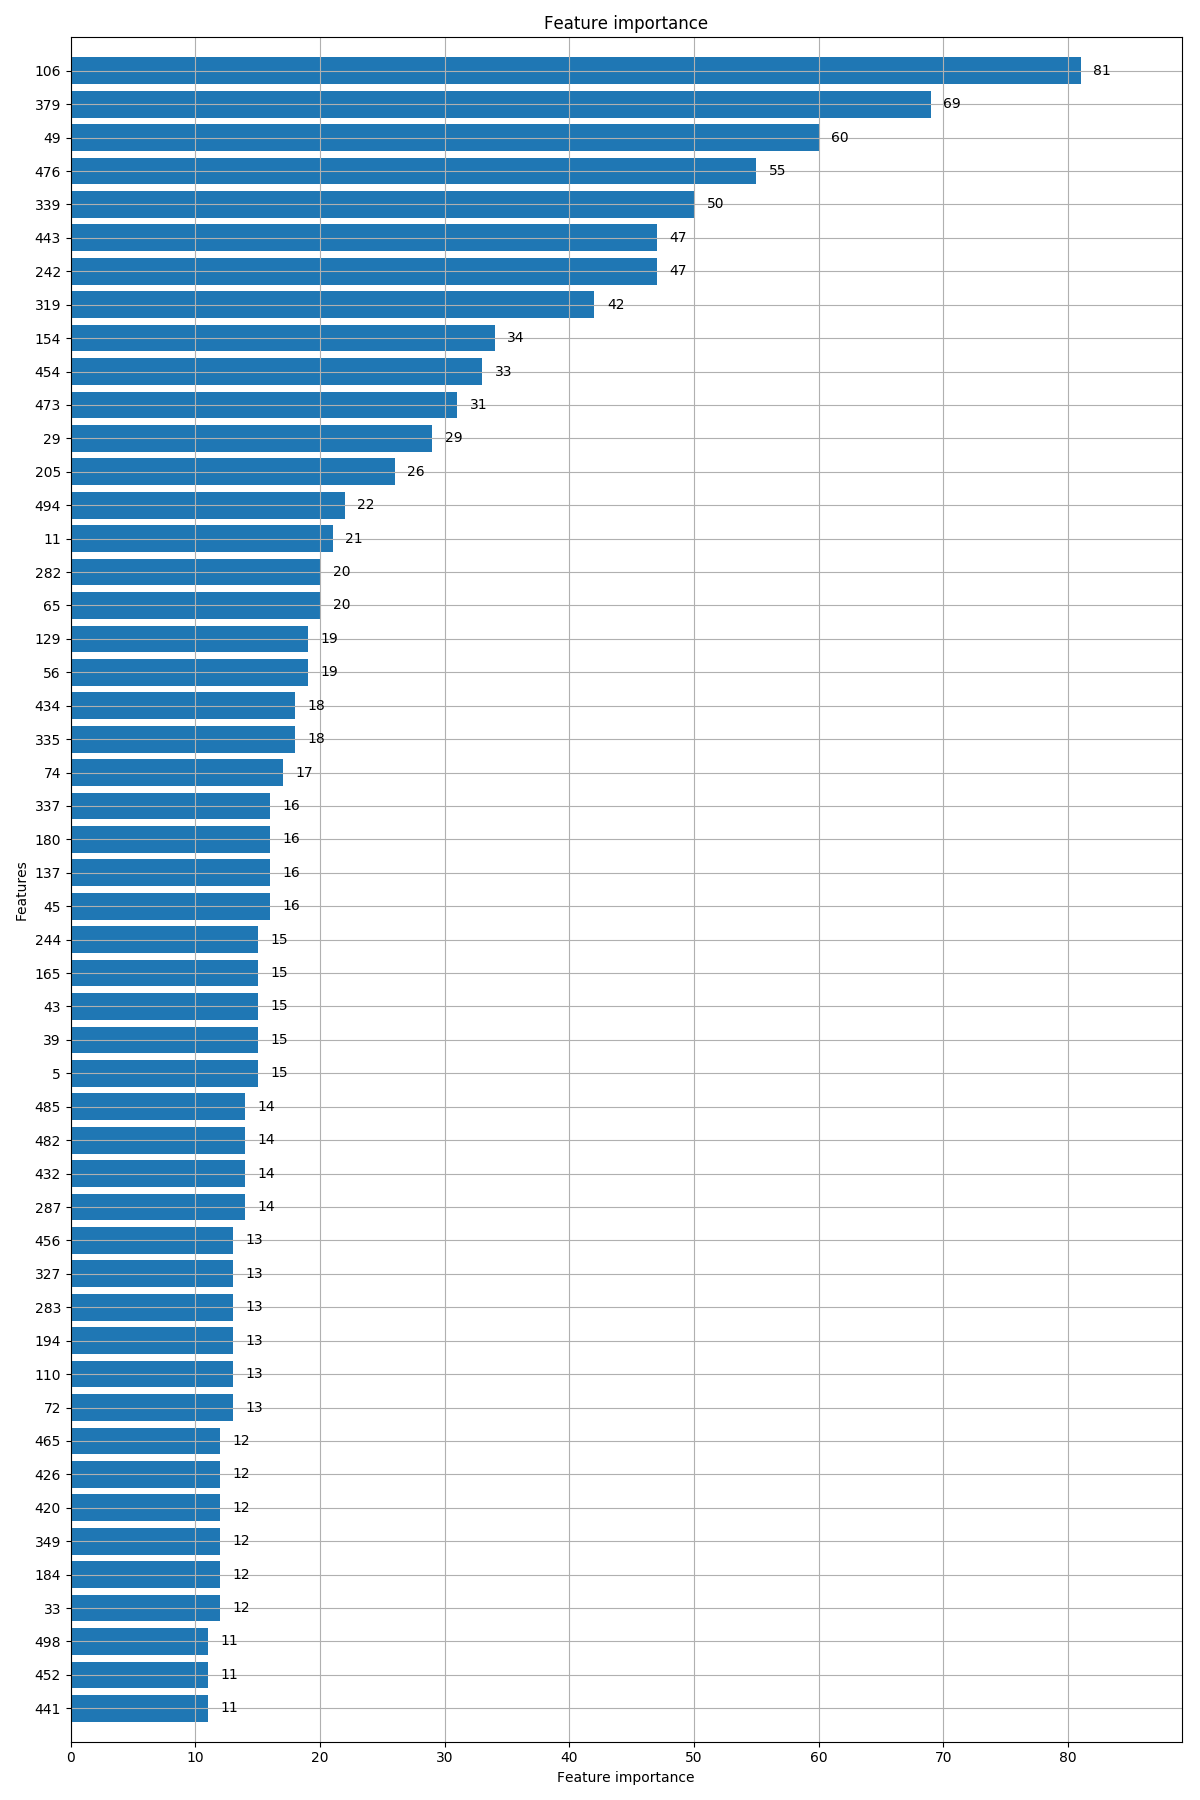
\includegraphics[width=0.85\textwidth]{../images/lightgbm-feature-importance.png}
            \caption{Istotność najważniejszych 30 cech dla modelu LightGBM}
            \label{fig:feature-importance-lightgbm}
        \end{figure}

        \section{Istotność cech dla modelu LightGBM}\label{appendix:feature-importance-xgboost}

        \begin{figure}[!h]
            \centering
            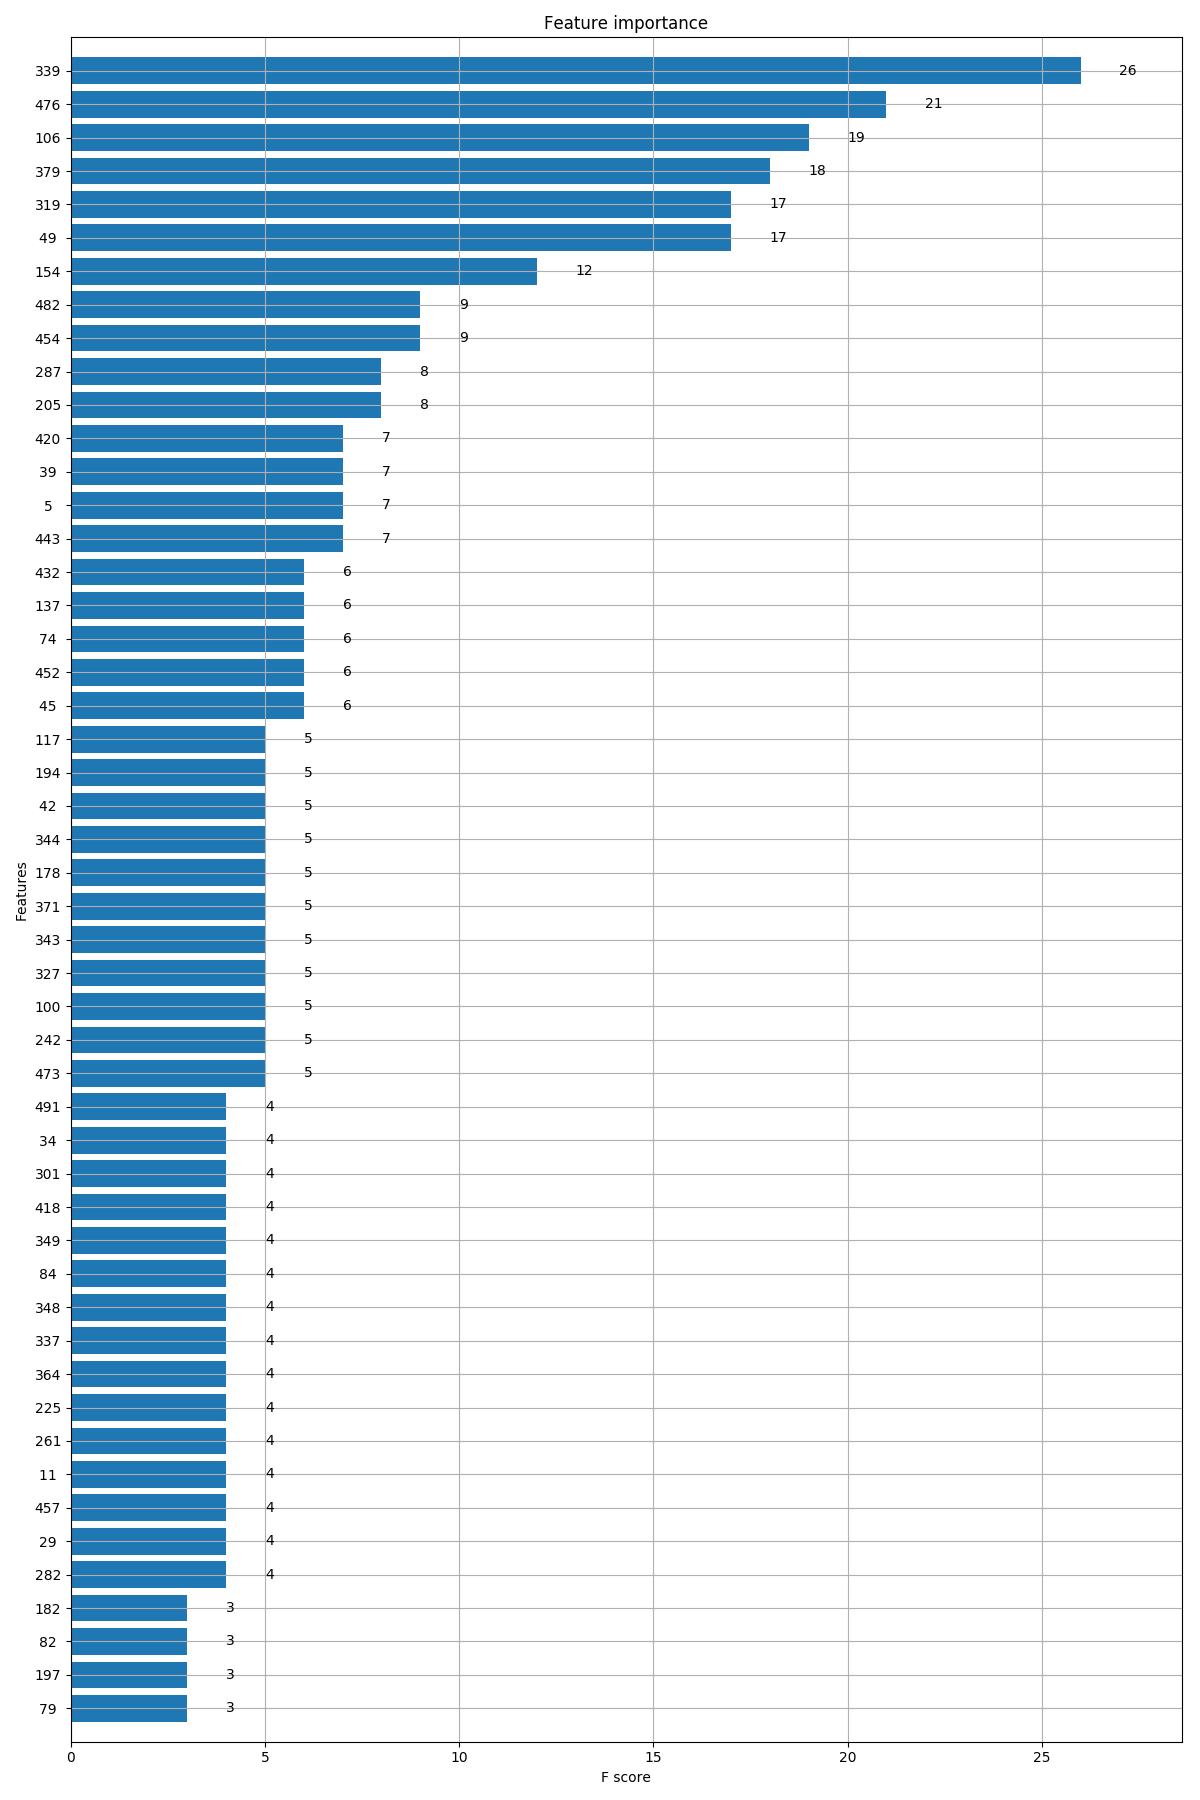
\includegraphics[width=0.85\textwidth]{../images/xgboost-feature-importance.png}
            \caption{Istotność najważniejszych 30 cech dla modelu XGBoost}
            \label{fig:feature-importance-xgboost}
        \end{figure}

    \end{appendices}

\end{document}
